\section{Introduction}\label{sec:introduction}
Your introduction goes here! Dummy citation: \cite{Alberts.2015}

\subsection{Dummy figure sub-section}\label{ssec:Dummyfiguresub-section}

\begin{figure}[h]%hbpt!H are options for figure placement
    \centering
    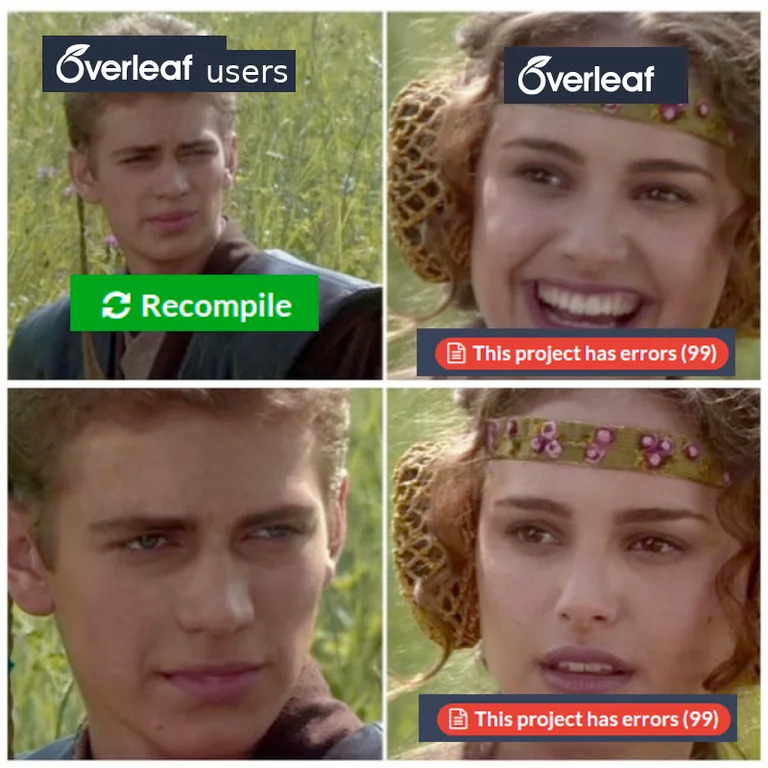
\includegraphics[width=.5\textwidth]{fig/overleaf.jpg}
    \caption{\textbf{A meaningful caption title.} This figure shows why compiling is always an option.}
    \label{fig:Ameaningfullcaption}
\end{figure}

\begin{table}[h]%hbpt!H are options for figure placement
    \centering
    \caption{\textbf{A dummy table.} You can use it as template for other tables. Remember caption goes on top because figure is bottom.}
    \label{tab:Thisisadummytable}
        \begin{tabular}{lcc} % l, r,c are options for alignments of a column, a | introduces vertical lines.
            \toprule
            \textbf{I}       &   \textbf{am}   &   \textbf{Head}    \\
            \midrule
            value   &   1    &   2       \\
            value   &   1    &   2       \\
            value   &   1    &   2       \\
            \bottomrule
        \end{tabular}
\end{table}


In the text we can do see: \Fref{fig:Ameaningfullcaption} or \sFref{fig:Ameaningfullcaption} and please look at \Tref{tab:Thisisadummytable} or \sTref{tab:Thisisadummytable}.
